%%%%%%%%%%%%%%%%%%%%%%%%%%%%%%%%%%%%%%%%%
% Focus Beamer Presentation
% LaTeX Template
% Version 1.0 (8/8/18)
%
% This template has been downloaded from:
% http://www.LaTeXTemplates.com
%
% Original author:
% Pasquale Africa (https://github.com/elauksap/focus-beamertheme) with modifications by 
% Vel (vel@LaTeXTemplates.com)
%
% Template license:
% GNU GPL v3.0 License
%
% Important note:
% The bibliography/references need to be compiled with bibtex.
%
%%%%%%%%%%%%%%%%%%%%%%%%%%%%%%%%%%%%%%%%%

%----------------------------------------------------------------------------------------
%	PACKAGES AND OTHER DOCUMENT CONFIGURATIONS
%----------------------------------------------------------------------------------------

\documentclass{beamer}

\usetheme{focus} % Use the Focus theme supplied with the template
% Add option [numbering=none] to disable the footer progress bar
% Add option [numbering=fullbar] to show the footer progress bar as always full with a slide count

% Uncomment to enable the ice-blue theme
%\definecolor{main}{RGB}{92, 138, 168}
%\definecolor{background}{RGB}{240, 247, 255}

%------------------------------------------------
\usepackage{booktabs} % Required for better table rules
\usepackage{amsgen,amsmath,amstext,amsbsy,amsopn,tikz,amssymb,tkz-linknodes}
\usepackage{pgfgantt}
\usepackage{subcaption} % For multiple images
\usepackage{subfiles} % Best loaded last in the preamble



\usetikzlibrary{arrows, automata}
\setbeamertemplate{caption}{\raggedright\insertcaption\par}

%----------------------------------------------------------------------------------------
%	 TITLE SLIDE
%----------------------------------------------------------------------------------------

\title{Solving The Art Gallery Problem Using Gradient Descent}

% \subtitle{Solving Job-Shop-like Problems with \\ Timed Automata}

\author{Georgiana Juglan}

\titlegraphic{
\includegraphics[scale=0.2, trim=-10cm -20cm 2cm -12cm]{Images/UU logo.png}} % Optional title page image, comment this line to remove it

\institute{Supervisor: Tillman Miltzow \\ Second Examiner: Frank Staals}

\date{\today}

%------------------------------------------------

\begin{document}

%------------------------------------------------

\begin{frame}
	\maketitle % Automatically created using the information in the commands above
\end{frame}

%----------------------------------------------------------------------------------------
%	 SECTION 1
%----------------------------------------------------------------------------------------

% \section{Section 1} % Section title slide, unnumbered

%------------------------------------------------

% \subfile{sections/1_jsp.tex}

\begin{frame}{The Art Gallery Problem}
	\begin{figure}
		\centering
		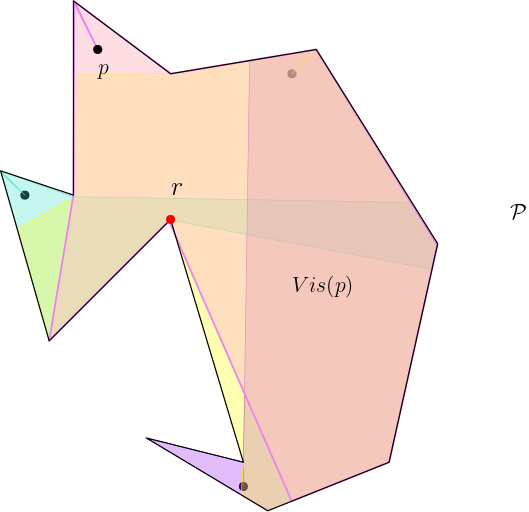
\includegraphics[width = 0.7\textwidth]{Images/p.png}
	\end{figure}
\end{frame}

% \begin{frame}{Previous Literature}
% 	\begin{itemize}
% 		\item approximation algorithms with ILPs
% 		\item no gradient descent so far
% 	\end{itemize}
% \end{frame}

\begin{frame}{Gradient Descent}
	\begin{figure}
		\centering
		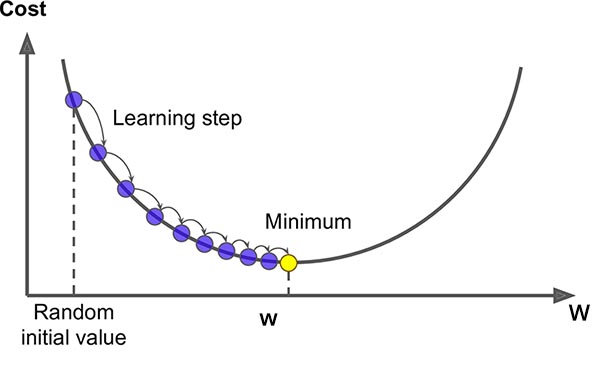
\includegraphics[width = 0.7\textwidth]{Images/external-content.duckduckgo.com.jpeg}
	\end{figure}
\end{frame}

\begin{frame}{Theory}
		\begin{columns}[T, onlytextwidth] % T for top align, onlytextwidth to suppress the margin between columns
		\column{0.65\textwidth}
			\begin{figure}
				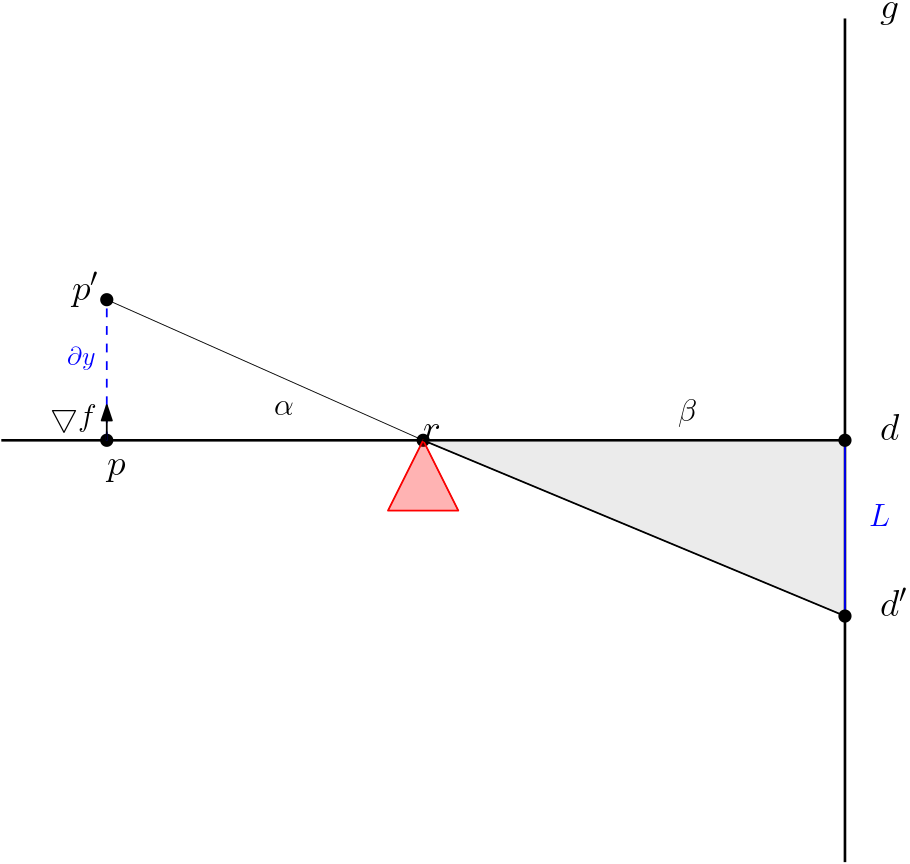
\includegraphics[width = \textwidth]{Images/gradient2.png}
			\end{figure}

		\column{0.25\textwidth}
			\centering
			$$\bigtriangledown f = \left(0, \frac{\beta^2}{2\alpha}\right)^\intercal$$
			$$p' = p + \alpha\bigtriangledown f,$$
			$$\alpha - \text{ learning rate}$$
	\end{columns}
\end{frame}

\begin{frame}{Practice}
	\begin{figure}[h!]
		\centering
		\begin{subfigure}{0.45\textwidth}
			\centering
			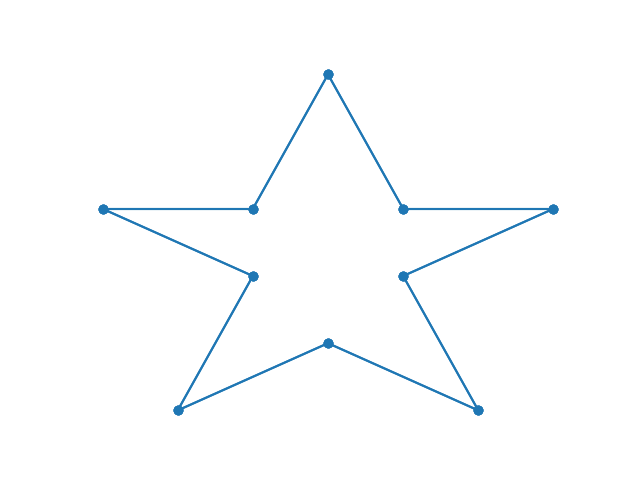
\includegraphics[width = 0.8\textwidth]{Images/pentagram.png}
			\caption{Star polygon.}
			\label{fig:star}
		\end{subfigure}
		\begin{subfigure}{0.45\textwidth}
			\centering
			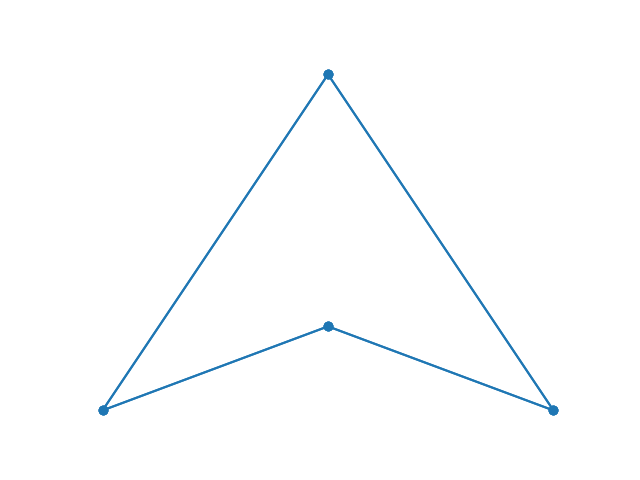
\includegraphics[width = 0.8\textwidth]{Images/concave_triangle.png}
			\caption{Arrowhead polygon.}
			\label{fig:concave}
		\end{subfigure}
		\begin{subfigure}{0.45\textwidth}
			\centering
			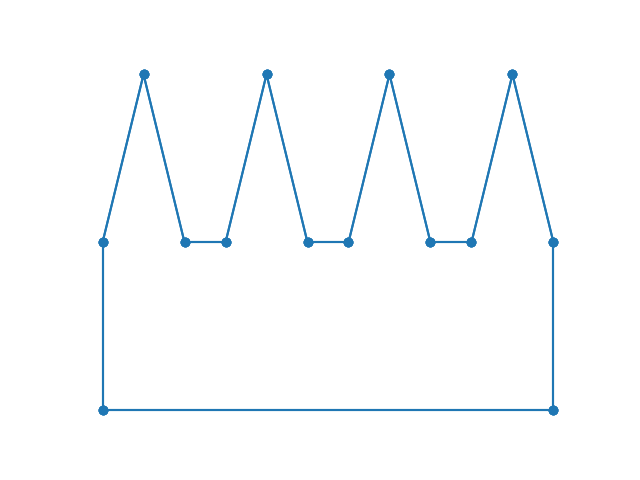
\includegraphics[width = 0.8\textwidth]{Images/comb.png}
			\caption{Comb polygon.}
			\label{fig:comb}
		\end{subfigure}
		\begin{subfigure}{0.45\textwidth}
			\centering
			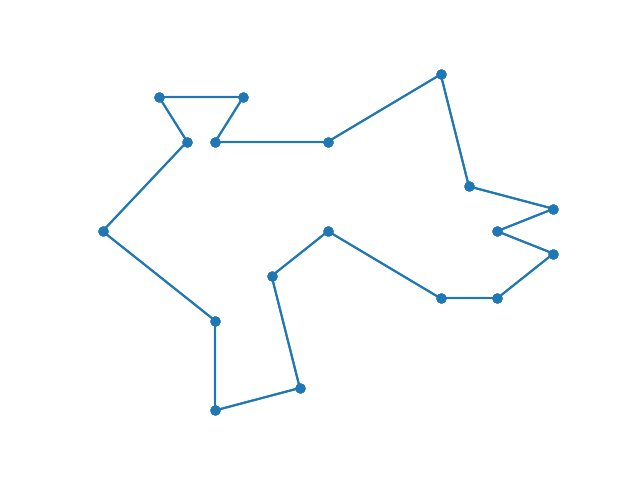
\includegraphics[width = 0.8\textwidth]{Images/random.png}
			\caption{Arbitrary polygon.}
			\label{fig:random}
		\end{subfigure}
		% \caption{Input polygons used for testing the algorithm.}
	\end{figure}
\end{frame}

% \begin{frame}{Practice}
% 	\begin{figure}
% 		\centering
% 		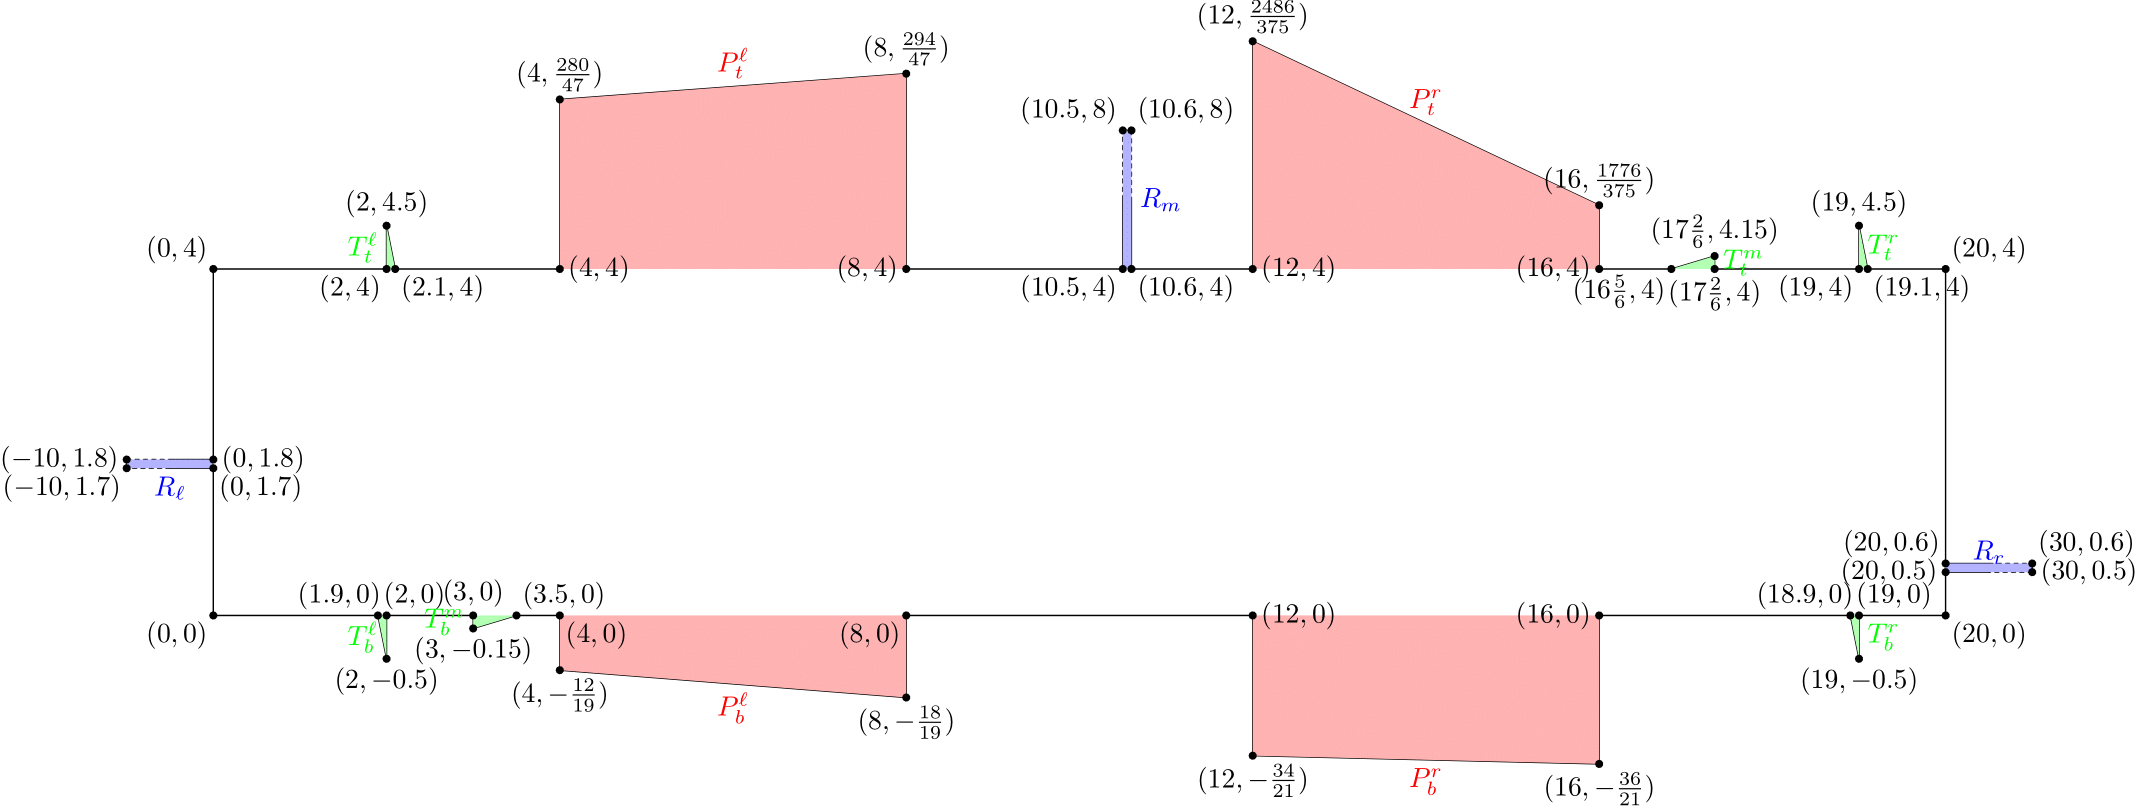
\includegraphics[width = \textwidth]{Images/fig-12-1.png}
% 		\caption{Irrational guards polygon \cite{abrahamsen2021art}.}
% 	\end{figure}
% \end{frame}

\begin{frame}{Practice}
	\begin{figure}[h!]
		\centering
		\begin{subfigure}{0.4\textwidth}
			\centering
			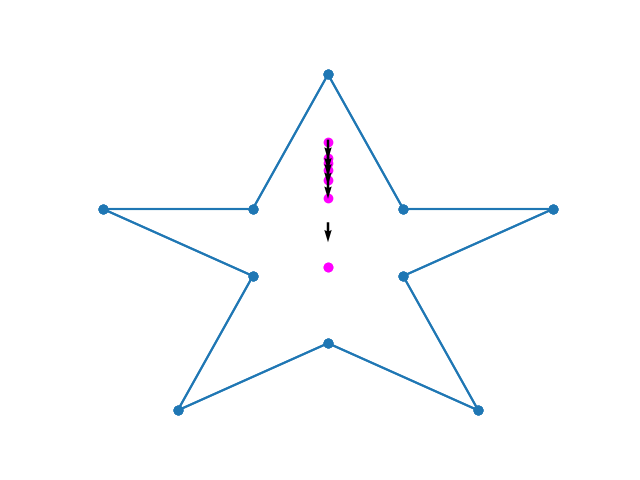
\includegraphics[width = 0.8\textwidth]{Images/pentagram_gradient.png}
			\caption{}
			\label{fig:star_gradient}
		\end{subfigure}
		\begin{subfigure}{0.4\textwidth}
			\centering
			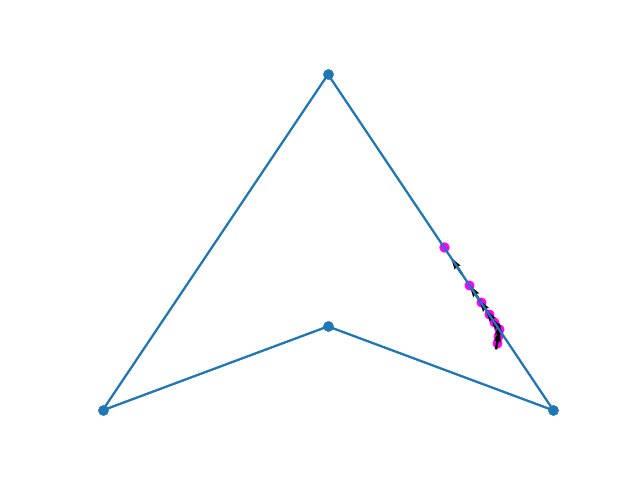
\includegraphics[width = 0.8\textwidth]{Images/concave_triangle_gradient.png}
			% \caption{Arrowhead polygon gradient example.}
			\caption{}
			\label{fig:concave_gradient}
		\end{subfigure}
		\begin{subfigure}{0.4\textwidth}
			\centering
			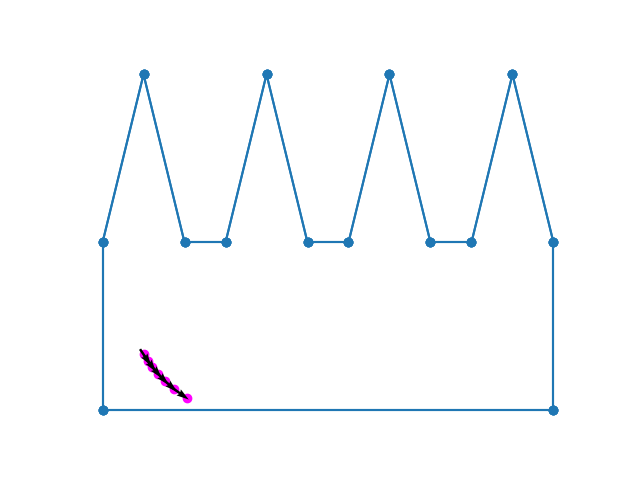
\includegraphics[width = 0.8\textwidth]{Images/comb_gradient.png}
			% \caption{Comb polygon gradient example.}
			\caption{}
			\label{fig:comb_gradient}
		\end{subfigure}
		\begin{subfigure}{0.4\textwidth}
			\centering
			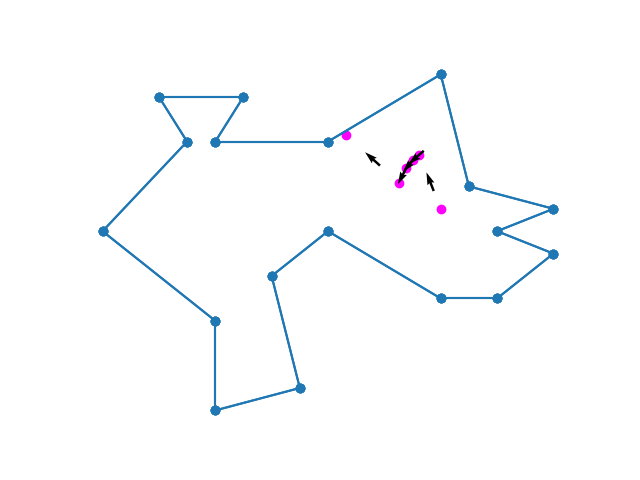
\includegraphics[width = 0.8\textwidth]{Images/random_gradient.png}
			% \caption{Arbitrary polygon gradient example.}
			\caption{}
			\label{fig:random_gradient}
		\end{subfigure}
		% \begin{subfigure}{\textwidth}
		% 	\centering
		% 	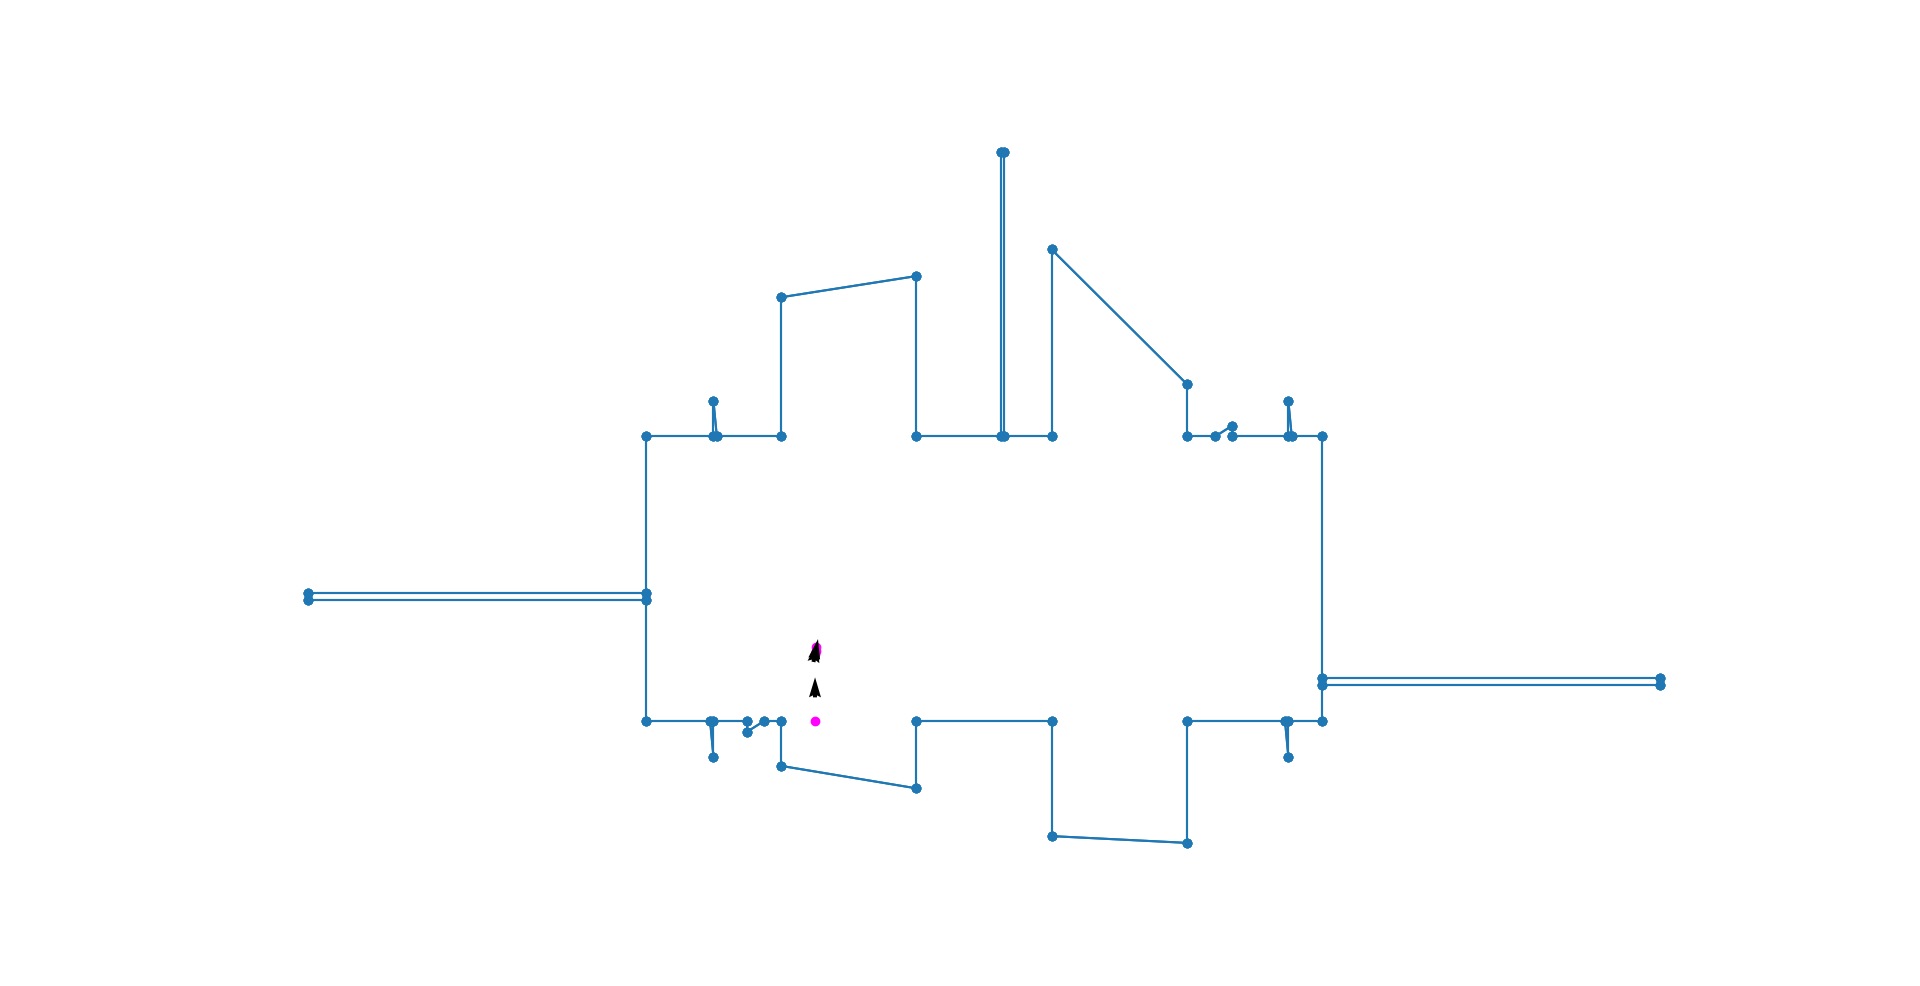
\includegraphics[width = \textwidth]{Images/love_gradient.png}
		% 	% \caption{Arbitrary polygon gradient example.}
		% 	\caption{Learning rate $l = 0.2$.}
		% 	\label{fig:love_gradient}
		% \end{subfigure}
		% \caption{Gradient descent examples with learning rate $l = 0.2$ on the test polygons.}
		\caption{Learning rate $l = 0.2$.}
		\label{fig:gradients}
	\end{figure}
\end{frame}

% \begin{frame}{Practice}
% 	\begin{figure}
% 		\centering
% 		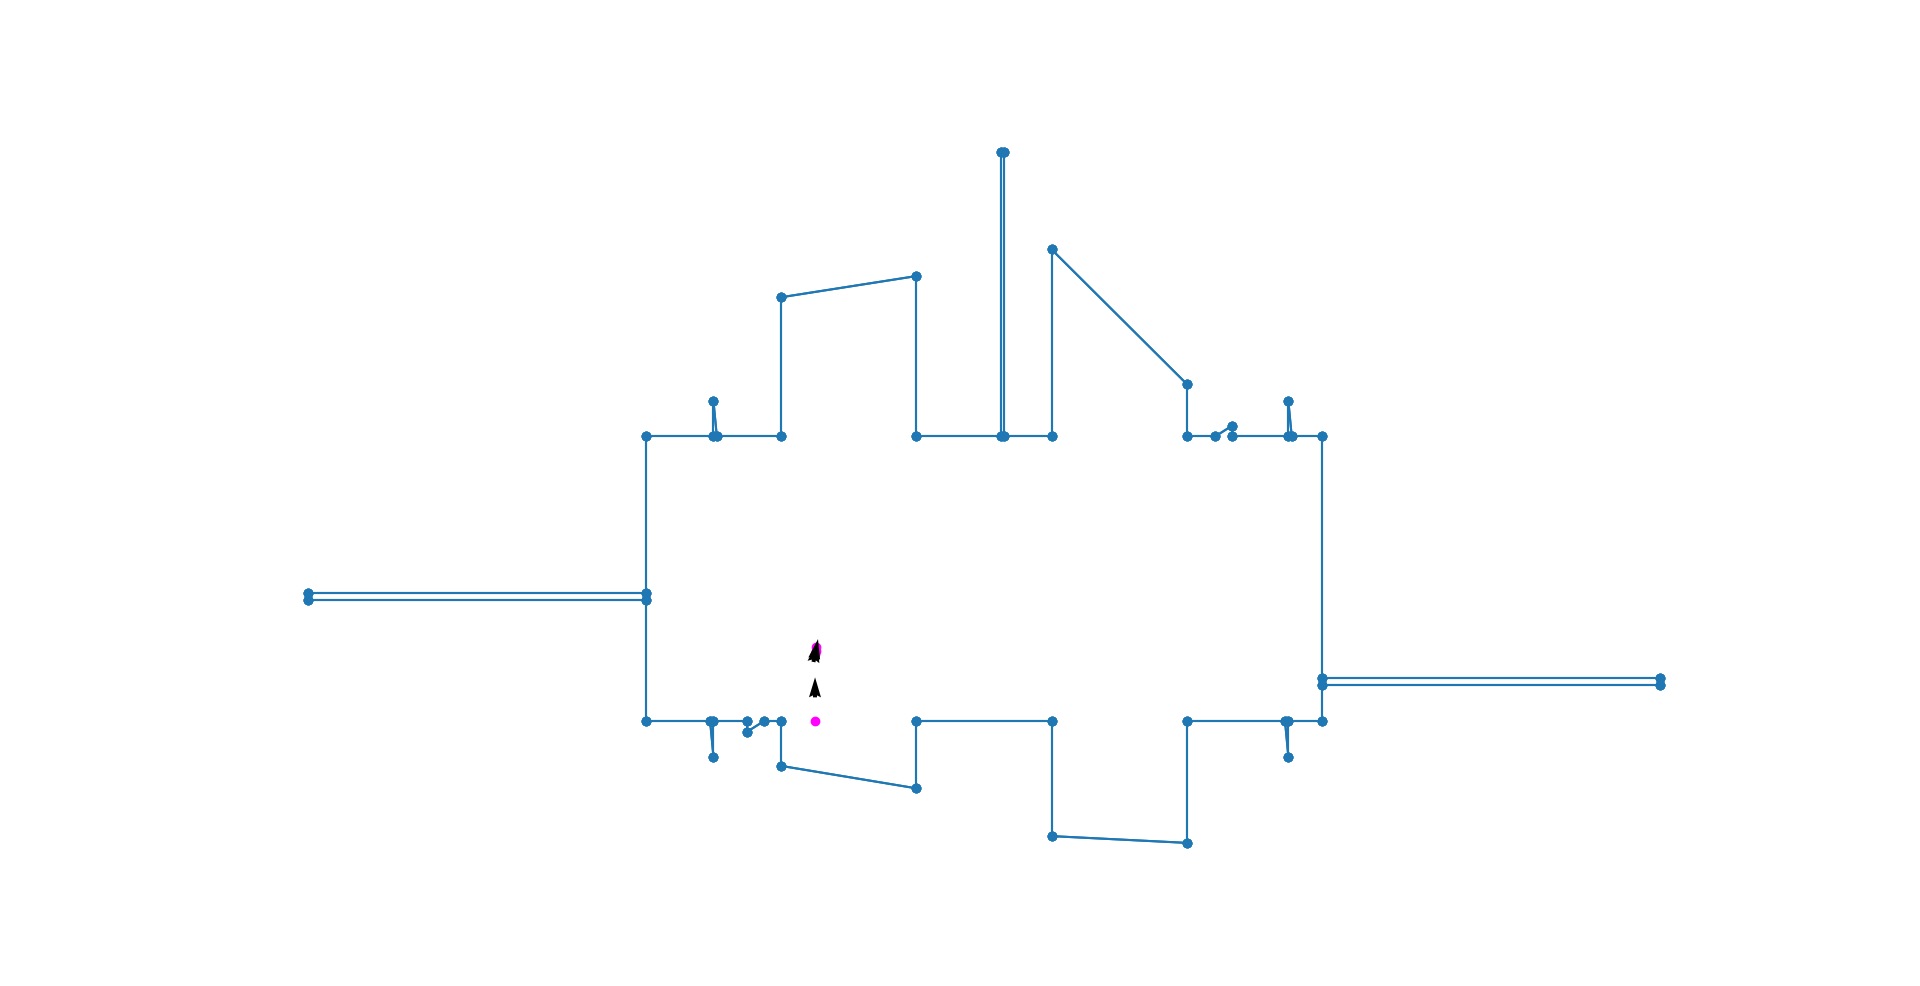
\includegraphics[width = \textwidth]{Images/love_gradient.png}
% 		\caption{Irrational guards polygon \cite{abrahamsen2021art} gradient example.}
% 	\end{figure}
% \end{frame}

\begin{frame}{Practice}
	\begin{figure}[h!]
		\centering
		\begin{subfigure}{0.45\textwidth}
			\centering
			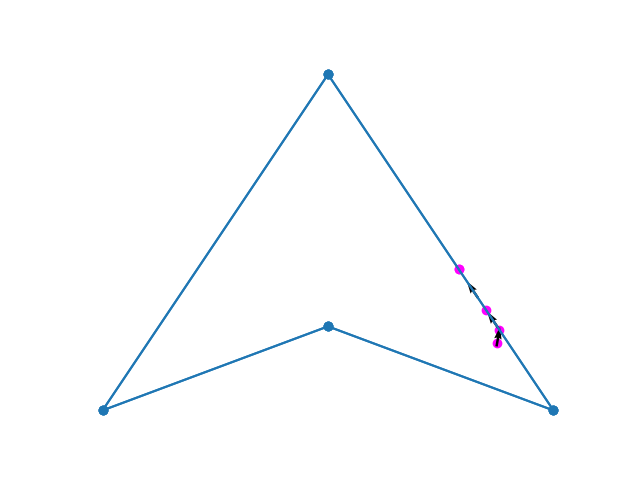
\includegraphics[width = 0.8\textwidth]{Images/concave_triangle_gradient_045.png}
			% \caption{Arrowhead polygon gradient with learning rate $l = 0.45$ example.}
			\caption{Learning rate $l = 0.45$.}
			\label{fig:concave_gradient_045}
		\end{subfigure}
		\begin{subfigure}{0.45\textwidth}
			\centering
			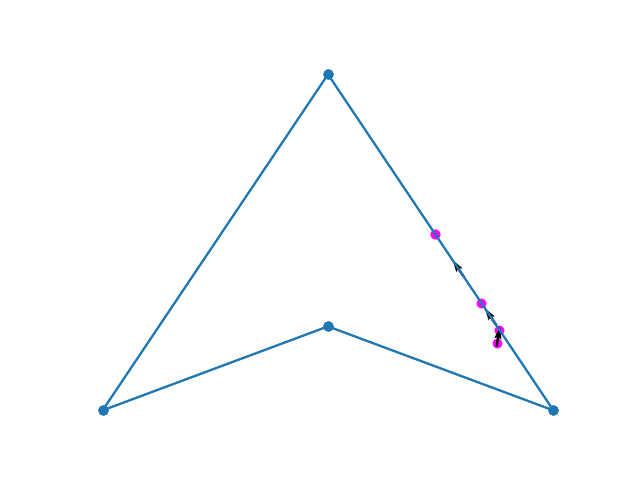
\includegraphics[width = 0.8\textwidth]{Images/concave_triangle_gradient_06.png}
			% \caption{Arrowhead polygon gradient with learning rate $l = 0.6$ example.}
			\caption{Learning rate $l = 0.6$.}
			\label{fig:concave_gradient_06}
		\end{subfigure}
		\begin{subfigure}{0.45\textwidth}
			\centering
			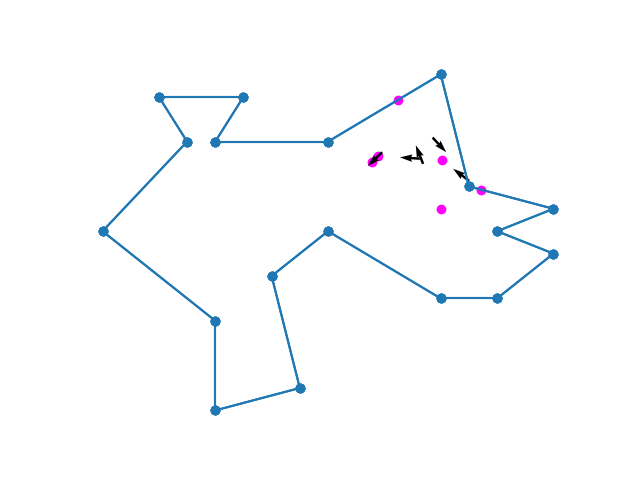
\includegraphics[width = 0.8\textwidth]{Images/random_gradient_045.png}
			% \caption{Arbitrary polygon gradient with learning rate $l = 0.45$ example.}
			\caption{Learning rate $l = 0.45$.}
			\label{fig:random_gradient_045}
		\end{subfigure}
		\begin{subfigure}{0.45\textwidth}
			\centering
			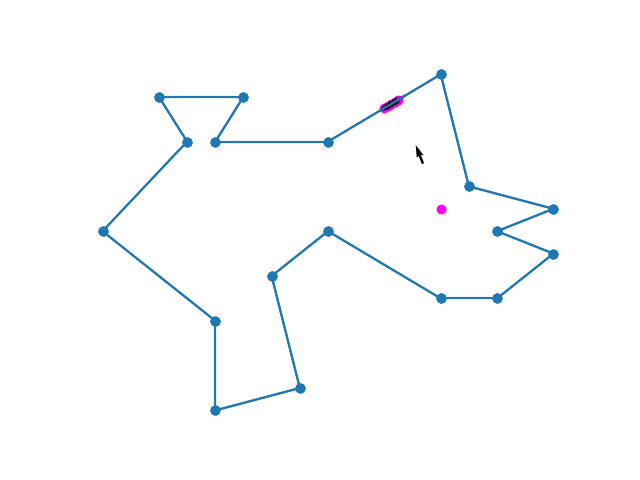
\includegraphics[width = 0.8\textwidth]{Images/random_gradient_06.png}
			% \caption{Arbitrary polygon gradient with learning rate $l = 0.6$ example.}
			\caption{Learning rate $l = 0.6$.}
			\label{fig:random_gradient_06}
		\end{subfigure}
		% \caption{Gradient descent examples with learning rate $l \in \{0.45, 0.6\}$ on the one-guard Arrowhead and multiple guards arbitrary input polygons.}
		\label{fig:multiple_gradients}
	\end{figure}
\end{frame}
\begin{frame}{Conclusion and Future Plans}
	\begin{itemize}
		\item gradient for multiple guards
		\pause
		\item gradient experiments (momentum, weighted momentum)
		\pause
		\item guard addition strategy
		\pause
		\item comparison with existing algorithms \cite{DBLP:journals/corr/abs-2007-06920}
	% 	\setlength{\itemsep}{0.5pt}
	% 	\item solve the Job-Shop Problem using Timed Automata
	% 	\item model the Travelling Salesman problem as an instance of the Single-Machine Shop problem
	% 	\item solve the Travelling Salesman Problem using Timed Automata 
	% 	\setlength{\itemsep}{10pt}
	% 	\item implementation
	% 	\setlength{\itemsep}{0.5pt}
	% 	\item complexity analysis
	% 	\item other methods for city grouping
	\end{itemize}
\end{frame}

%------------------------------------------------

% \begin{frame}[plain]{Plain Slide}
% 	% This is a slide with the plain style and it is numbered.
% \end{frame}

% %------------------------------------------------

% \begin{frame}[t]
% 	This slide has an empty title and is aligned to top.
% \end{frame}

% %------------------------------------------------

% \begin{frame}[noframenumbering]{No Slide Numbering}
% 	This slide is not numbered and is citing reference \cite{knuth74}.
% \end{frame}

% %------------------------------------------------

% \begin{frame}{Typesetting and Math}
% 	The packages \texttt{inputenc} and \texttt{FiraSans}\footnote{\url{https://fonts.google.com/specimen/Fira+Sans}}\textsuperscript{,}\footnote{\url{http://mozilla.github.io/Fira/}} are used to properly set the main fonts.
% 	\vfill
% 	This theme provides styling commands to typeset \emph{emphasized}, \alert{alerted}, \textbf{bold}, \textcolor{example}{example text}, \dots
% 	\vfill
% 	\texttt{FiraSans} also provides support for mathematical symbols:
% 	\begin{equation*}
% 		e^{i\pi} + 1 = 0.
% 	\end{equation*}
% \end{frame}

% %----------------------------------------------------------------------------------------
% %	 SECTION 2
% %----------------------------------------------------------------------------------------

% \section{Section 2}

% %------------------------------------------------

% \begin{frame}{Blocks}
% 	These blocks are part of 1 slide, to be displayed consecutively.
% 	\begin{block}{Block}
% 		Text.
% 	\end{block}
% 	\pause % Automatically creates a new "page" split between the above and above + below
% 	\begin{alertblock}{Alert block}
% 		Alert \alert{text}.
% 	\end{alertblock}
% 	\pause % Automatically creates a new "page" split between the above and above + below
% 	\begin{exampleblock}{Example block}
% 		Example \textcolor{example}{text}.
% 	\end{exampleblock}
% \end{frame}

%------------------------------------------------

% \begin{frame}{Timed Automaton Example}
% 	\begin{columns}
		
% \end{frame}

%------------------------------------------------

% \begin{frame}{Lists}
% 	\begin{columns}[T, onlytextwidth] % T for top align, onlytextwidth to suppress the margin between columns
% 		\column{0.33\textwidth}
% 			Items:
% 			\begin{itemize}
% 				\item Item 1
% 				\begin{itemize}
% 					\item Subitem 1.1
% 					\item Subitem 1.2
% 				\end{itemize}
% 				\item Item 2
% 				\item Item 3
% 			\end{itemize}
		
% 		\column{0.33\textwidth}
% 			Enumerations:
% 			\begin{enumerate}
% 				\item First
% 				\item Second
% 				\begin{enumerate}
% 					\item Sub-first
% 					\item Sub-second
% 				\end{enumerate}
% 				\item Third
% 			\end{enumerate}
		
% 		\column{0.33\textwidth}
% 			Descriptions:
% 			\begin{description}
% 				\item[First] Yes.
% 				\item[Second] No.
% 			\end{description}
% 	\end{columns}
% \end{frame}

% %------------------------------------------------

% \begin{frame}{Table}
% 	\begin{table}
% 		\centering % Centre the table on the slide
% 		\begin{tabular}{l c}
% 			\toprule
% 			Discipline & Avg. Salary \\
% 			\toprule
% 			\textbf{Engineering} & \textbf{\$66,521} \\
% 			Computer Sciences & \$60,005\\
% 			Mathematics and Sciences & \$61,867\\
% 			Business & \$56,720\\
% 			Humanities \& Social Sciences & \$56,669\\
% 			Agriculture and Natural Resources & \$53,565\\
% 			Communications & \$51,448\\
% 			\midrule
% 			\textbf{Average for All Disciplines} & \textbf{\$58,114}\\
% 			\bottomrule
% 		\end{tabular}
% 	\caption{Table caption}
% 	\end{table}
% \end{frame}

% %------------------------------------------------

% \begin{frame}[focus]
% 	Thanks for using \textbf{Focus}!
% \end{frame}

%----------------------------------------------------------------------------------------
%	 CLOSING/SUPPLEMENTARY SLIDES
%----------------------------------------------------------------------------------------

\appendix

\begin{frame}{References}
	% \nocite{*} % Display all references regardless of if they were cited
	\bibliography{example.bib}
	\bibliographystyle{plain}
\end{frame}

% %------------------------------------------------

% \begin{frame}{Backup Slide}
% 	This is a backup slide, useful to include additional materials to answer questions from the audience.
% 	\vfill
% 	The package \texttt{appendixnumberbeamer} is used to refrain from numbering appendix slides.
% \end{frame}

%----------------------------------------------------------------------------------------

\end{document}
